\documentclass[10pt]{beamer}

\usepackage[utf8]{inputenc}
\usepackage{graphicx}
% \usepackage{bookman}
\usepackage{amsmath}

\usetheme{Madrid}
% \usecolortheme{beaver}

\providecommand{\main}{.}
\graphicspath{{img/}}

\title[INDOOR LOCALIZATION SYSTEM]{DESIGN AND IMPLEMENTATION OF INDOOR LOCALIZATION SYSTEM USING UWB AND WIRELESS MESH NETWORK}
\subtitle{Graduation Thesis}
\author[Ngo Van Tuan - 1613861]{Student: Ngo Van Tuan - 1613861\\
Supervisor: Dr. Vo Que Son}
\institute[HCMUT] % (optional)
{
  \inst{1}
%   VIETNAM NATIONAL UNIVERSITY HO CHI MINH CITY\\
%   HO CHI MINH CITY UNIVERSITY OF TECHNOLOGY\\
  FACULTY OF ELECTRICAL AND ELECTRONICS  ENGINEERING\\
  DEPARTMENT OF TELECOMMUNICATIONS ENGINEERING
}
\date{January 26, 2021}
\logo{
\includegraphics[height=1cm]{logoBK.png}}

\begin{document}

\frame{\titlepage}

\begin{frame}
    \frametitle{Table of Contents}
    \tableofcontents
\end{frame}

\AtBeginSection[]
{
  \begin{frame}
    \frametitle{Table of Contents}
    \tableofcontents[currentsection]
  \end{frame}
}

\section{Introduction}

\begin{frame}
\frametitle{Introduction: Outdoor vs Indoor Localization}
\begin{columns}
\column{0.5\textwidth}
Advantages of GPS:
\begin{itemize}
    \item Almost available anywhere
    \item Free to use
    \item Get calibrated by its own
    \item Provide location based info
\end{itemize}
\begin{figure}[h]
    \begin{center}
        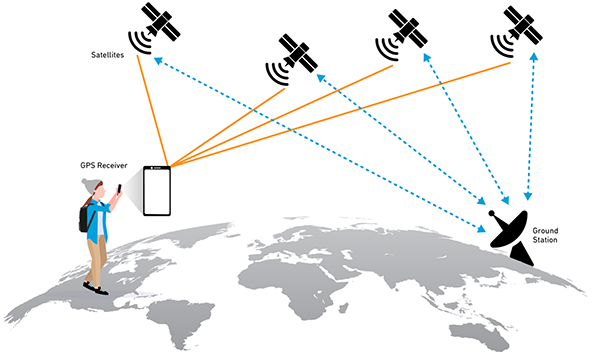
\includegraphics[width=1\textwidth]{gps.png}
    \end{center}
    \caption{Global Positioning System}
    \label{fig:gps}
\end{figure}
\column{0.5\textwidth}
Disadvantages of GPS:
\begin{itemize}
    \item Do not pierce through the solid walls or structures
    \item Not accurate enough for indoor applications
    % \item Not quick enough for realtime applications
\end{itemize}
\begin{figure}[h]
    \begin{center}
        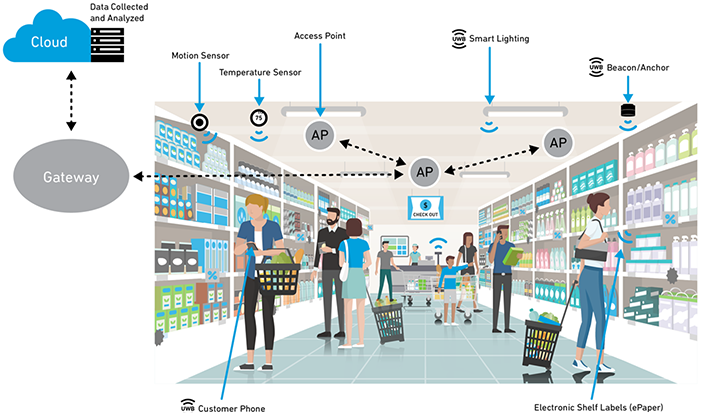
\includegraphics[width=1\textwidth]{ips.png}
    \end{center}
    \caption{Indoor Positioning System}
    \label{fig:ips}
\end{figure}
\end{columns}
\end{frame}

\begin{frame}
    \frametitle{Introduction: Thesis Objective}    
    \begin{columns}
        \column{0.4\textwidth}
    \begin{itemize}
        \item Design and implement an indoor localization system using UWB
        \item Build a system to manage and control the localization
        system based on Bluetooth mesh network
        \item Provide IoT services for remote control and self-identification
    \end{itemize}
    \column{0.6\textwidth}
    \begin{figure}[H]
        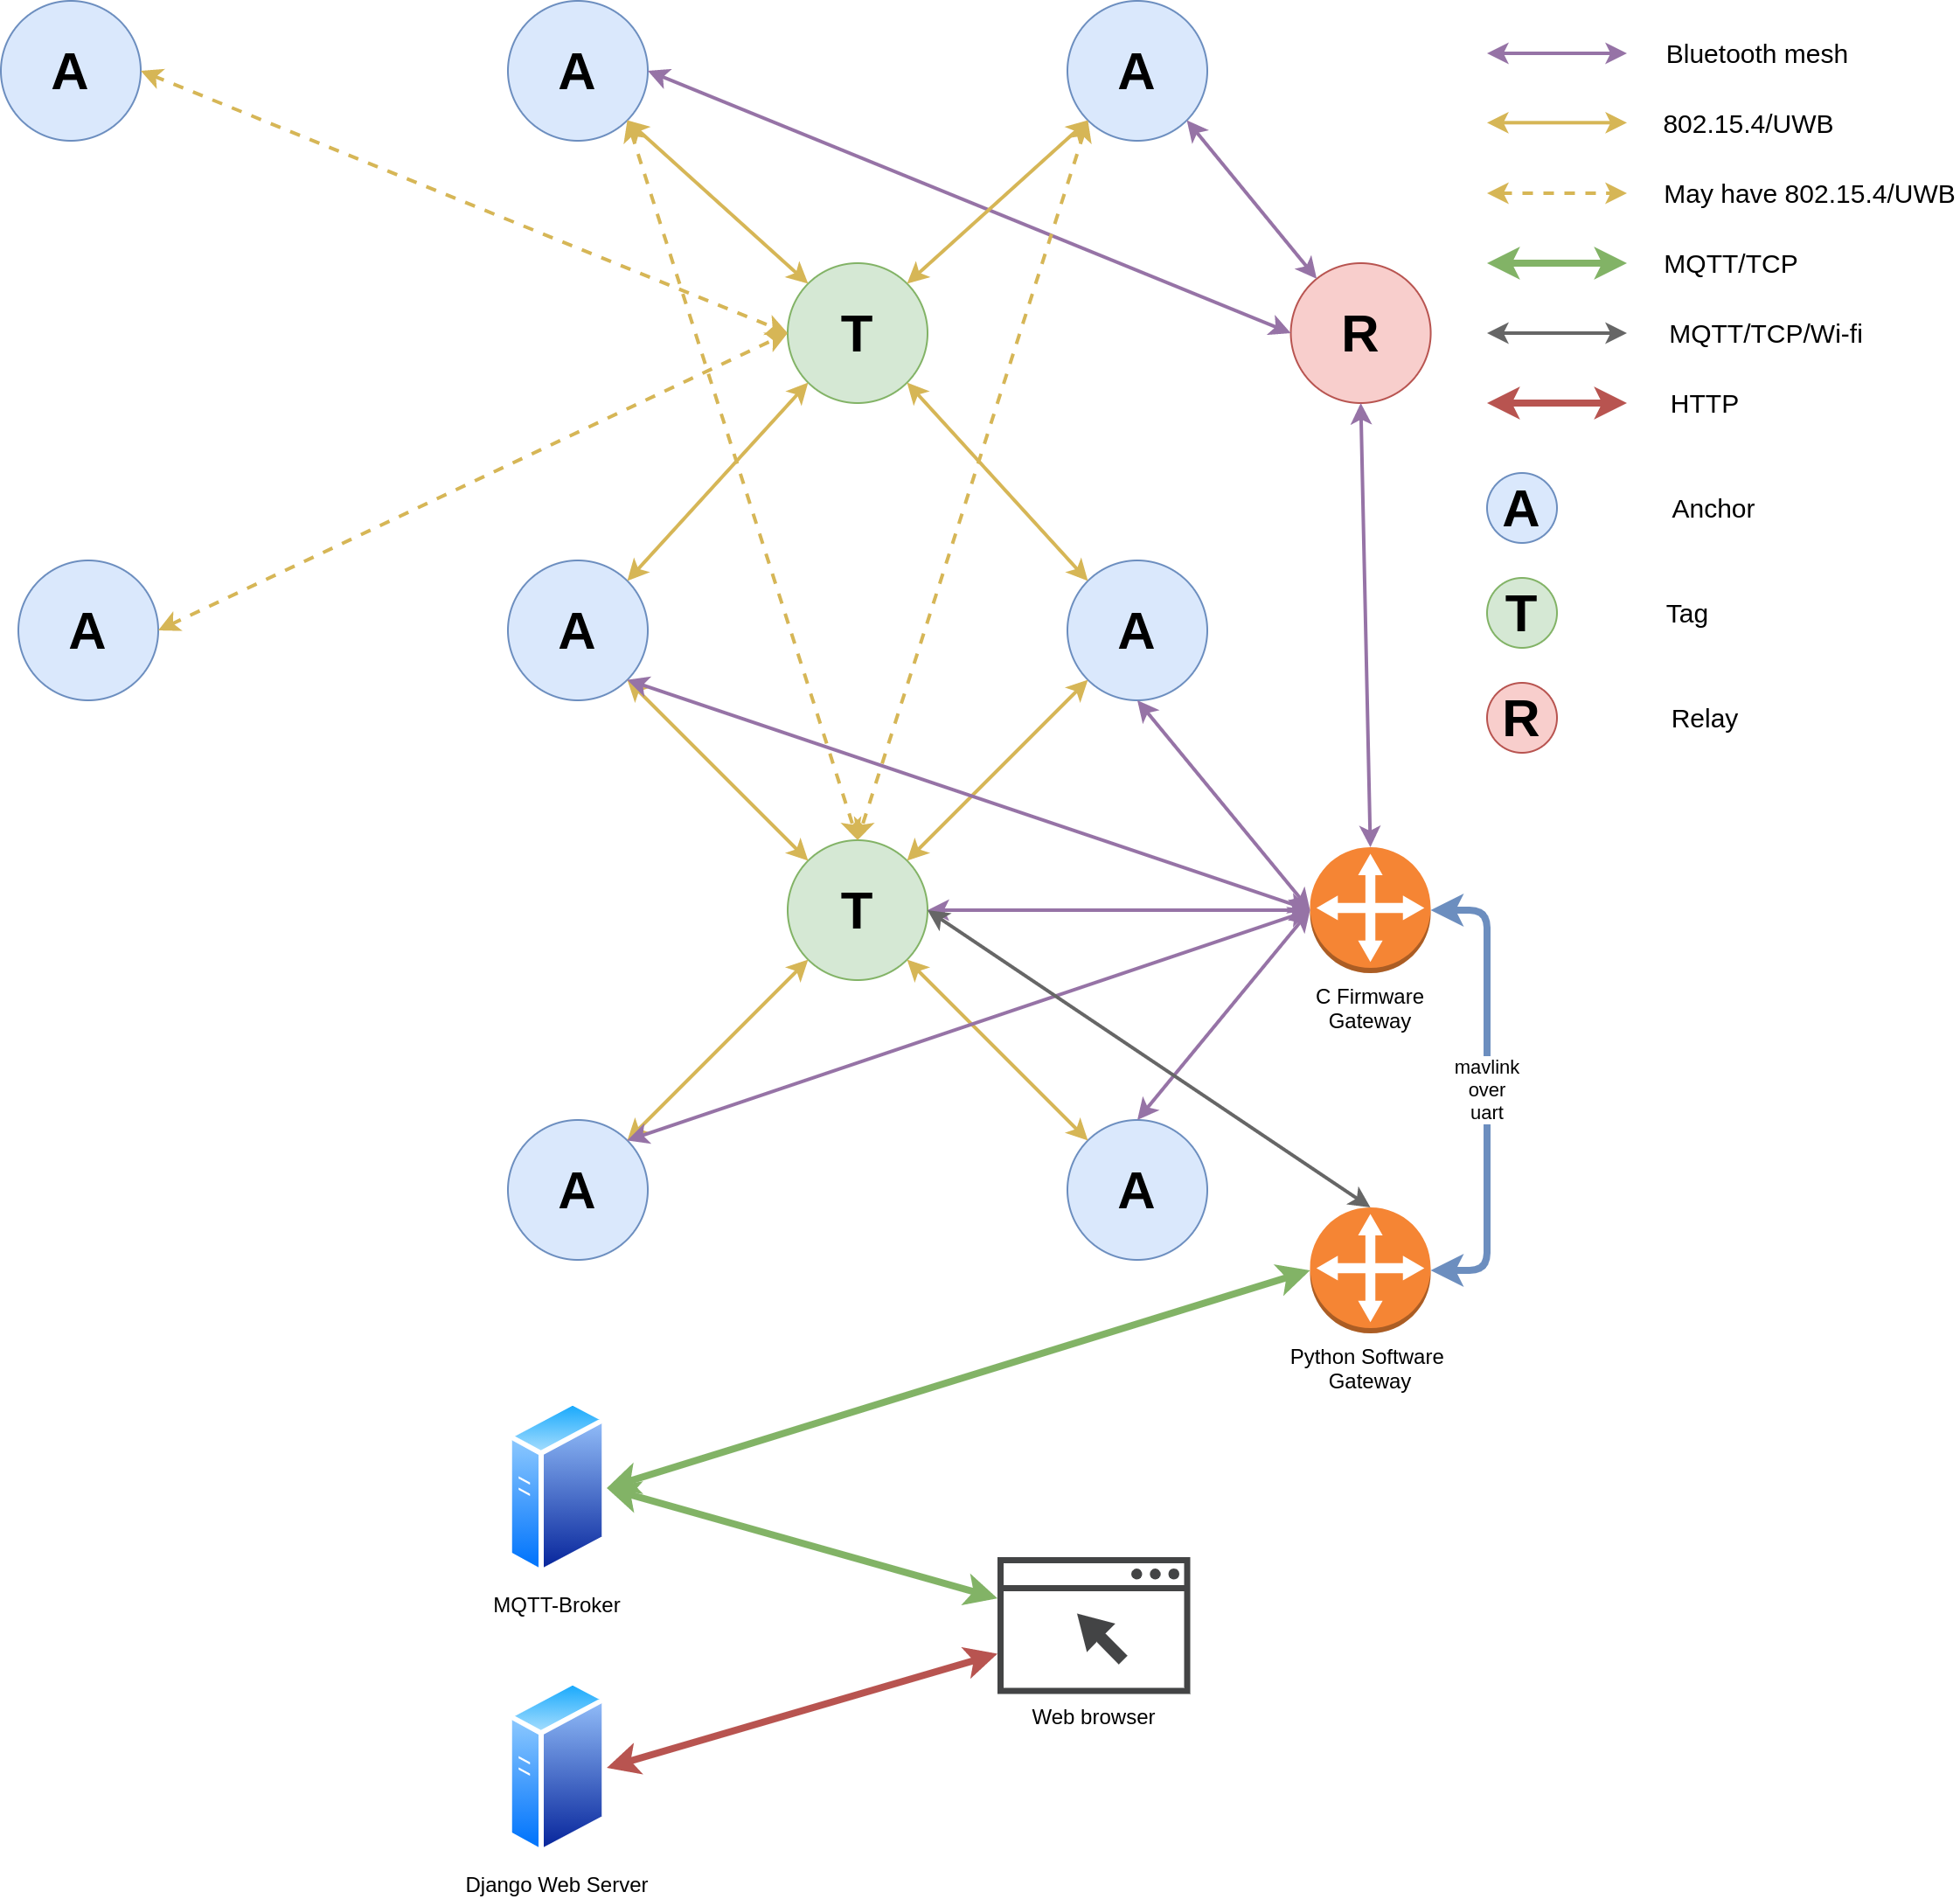
\includegraphics[width=0.8\textwidth]{system_overview.png}
        \caption{System overview}
        \label{fig:system_overview}
    \end{figure}
    \end{columns}
\end{frame}

\begin{frame}
    \frametitle{Introduction: Ultra-Wideband}
    Definition of Ultra-Wideband signal:
\begin{columns}
    \column{0.3\textwidth}
    \begin{equation}
        B=(f\textsubscript{H} - f\textsubscript{L})
    \end{equation}
    \begin{equation}
        f\textsubscript{c} = \frac{f\textsubscript{H} + f\textsubscript{L}}{2}\
    \end{equation} 

    \begin{equation}
        B\textsubscript{frac} =\frac{B}{f\textsubscript{c}} = \frac{2(f\textsubscript{H} - f\textsubscript{L})}{f\textsubscript{H} + f\textsubscript{L}}
    \end{equation}

    \column{0.7\textwidth}
    \begin{figure}[H]
    \centering
    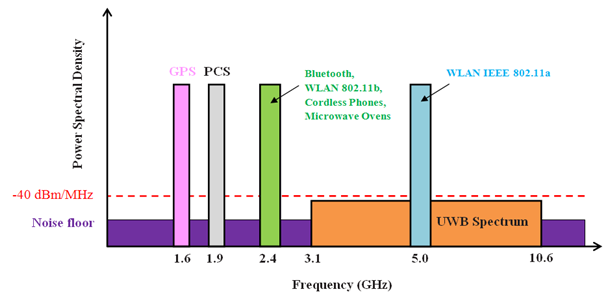
\includegraphics[width=1\textwidth]{uwb_versus_other_radio_communication_systems.png}
    \caption{UWB}
    \label{fig:uwb_versus_other_radio_communication_systems}
    \end{figure}
\end{columns}
Federal Communication Commission (FCC) has defined UWB signal:
\begin{itemize} 
    \item Absolute bandwidth greater than or equal 500Mhz, or
    \item $B$\textsubscript{frac} larger than 0.2
\end{itemize}
\end{frame}

\begin{frame}
    \frametitle{Introduction: Why UWB + DWM1001?}
    Advantages of UWB:
    \begin{itemize}
        \item Potentially low complexity and low cost
        \item Noise like signal
        \item Resistant to multi-path and jamming
        \item Good time-domain resolution allowing for localization application
    \end{itemize}
    \begin{columns}
        \column{0.3\textwidth}
        \begin{figure}[H]
            \centering
            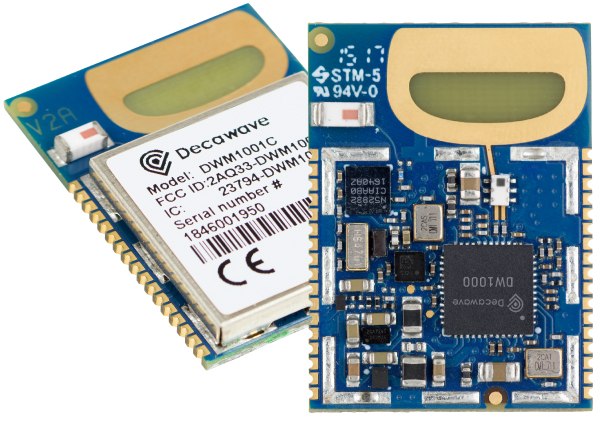
\includegraphics[width=1\textwidth]{DWM1001_Module_ProdPage_600x430.jpg}
            \caption{DWM1001 Module}
            \label{fig:DWM1001_Module_ProdPage_600x430}
        \end{figure}
        \column{0.7\textwidth}
        \begin{figure}[H]
            \centering
            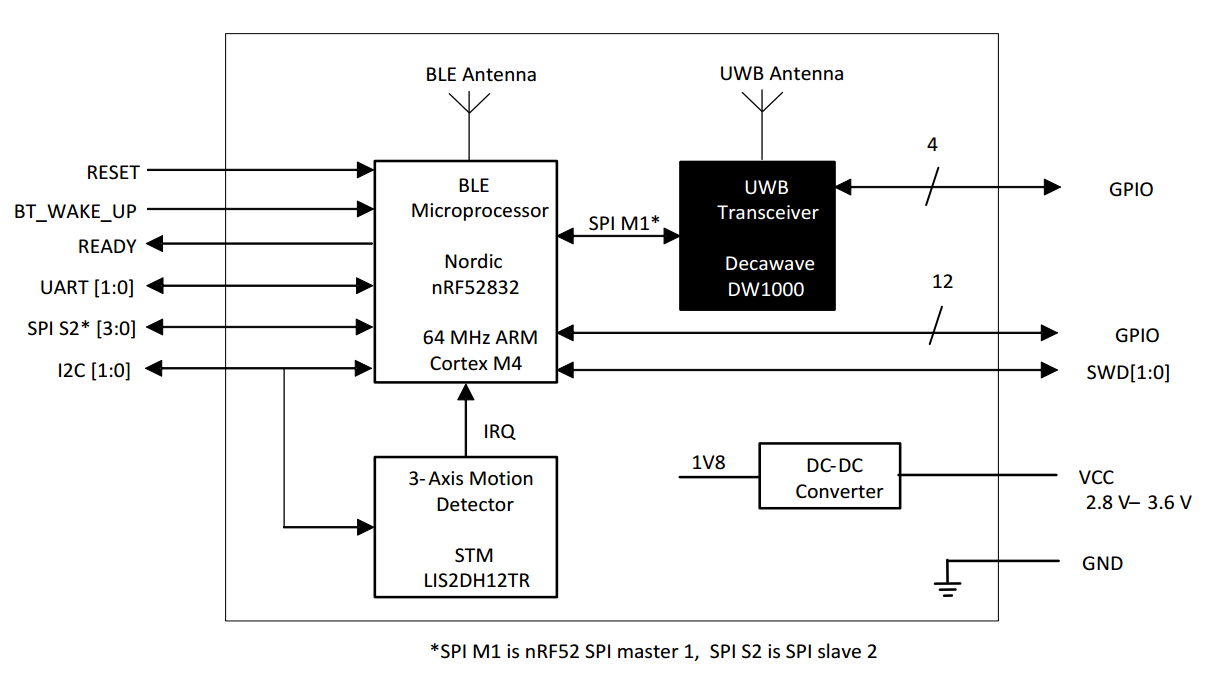
\includegraphics[width=1\textwidth]{dwm1001_block_diagram.png}
            \caption{DWM1001 block diagram}
            \label{fig:dwm1001_block_diagram}
        \end{figure}
    \end{columns}
\end{frame}

\section{Position estimation}

\begin{frame}
    \frametitle{Position estimation: Two-Way Ranging}
    Time of Fight formula: 
    \begin{equation}
        tof = \frac{1}{2} ((tt2 - tt1) - (ta2 - ta1))
        \label{eqn:pos_est_twr_tof}
    \end{equation}
    \begin{columns}
        \column{0.3\textwidth}
        \begin{figure}[H]
            \centering
            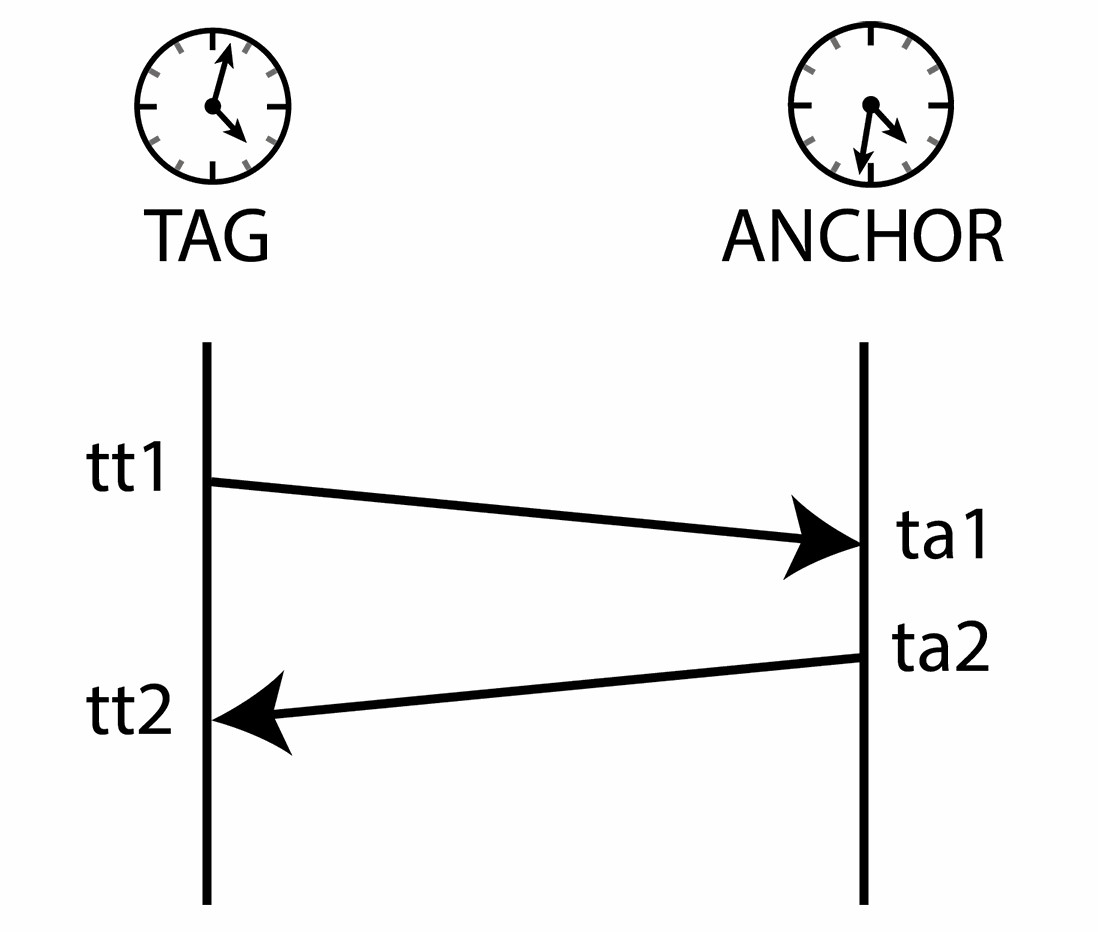
\includegraphics[width=1\textwidth]{twr_protocol.png}
            \caption{TWR}
            \label{fig:twr_anchor_and_tag}
        \end{figure}
        \column{0.7\textwidth}
        \begin{figure}[H]
            \centering
            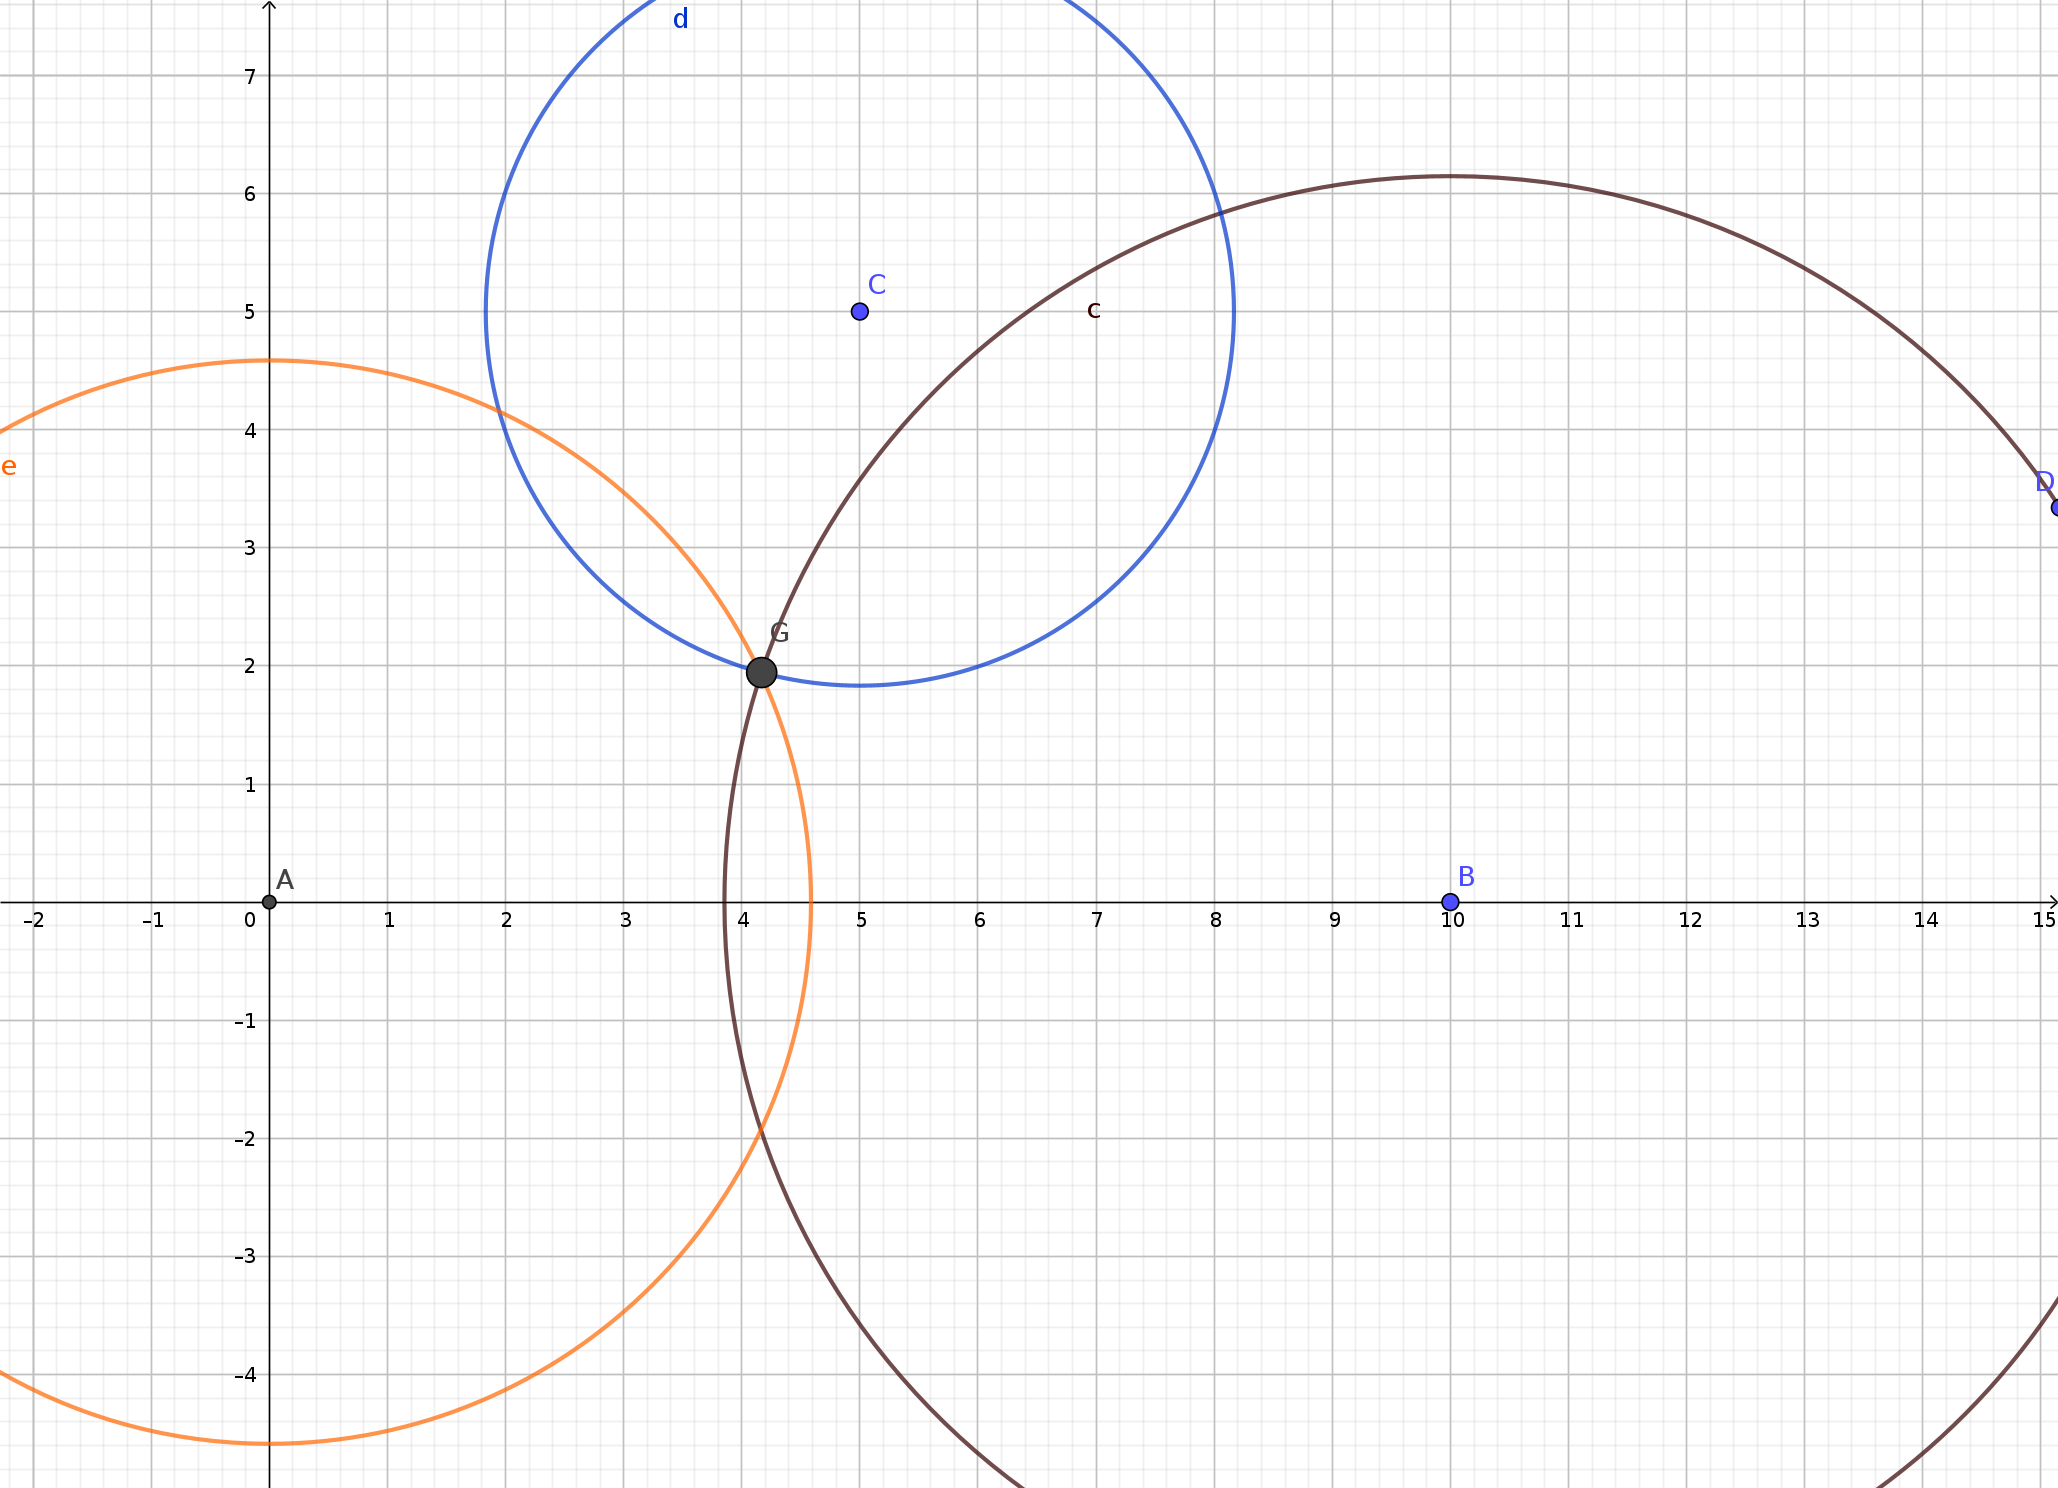
\includegraphics[width=0.8\textwidth]{twr.png}
            \caption{Localization using TWR}
            \label{fig:twr_trilateration}
        \end{figure}
    \end{columns}
\end{frame}

\begin{frame}
    \frametitle{Position estimation: Multilateration in 3D Euclidean Space}
    \begin{columns}
    \column{0.5\textwidth}
        \begin{columns}
            \column{0.2\textwidth}
            Anchors:
            \column{0.8\textwidth}
            $A_1(0,0,0)$\\
            $A_2(x_2,0,0)$\\
            $A_3(x_3,y_3,0)$
        \end{columns}
        \begin{columns}
            \column{0.2\textwidth}
            Tag:
            \column{0.8\textwidth}
            $T(x,y,z)$
        \end{columns}

        % \begin{equation}
        %     \begin{split}
        %         &A_1(0,0,0)\\
        %         &A_2(x_2,0,0)\\
        %         &A_3(x_3,y_3,0)
        %     \end{split}
        %     \label{eqn:simplified_multilateration_x}
        % \end{equation}

        \begin{equation}
            \begin{split}
                d_1 = | T - A_1| \\
                d_2 = | T - A_2| \\
                d_3 = | T - A_3|
            \end{split}
        \end{equation}
        \begin{subequations}
            \begin{align}
                & x^2 + y^2 + z^2 = d_1^2 \label{eqn:d1_t_a_a}\\
                & (x-x_2)^2 + y^2 + z^2 = d_2^2 \label{eqn:d1_t_a_b}\\
                & (x-x_3)^2 + (y-y_3)^2 + z^2 = d_3^2 \label{eqn:d1_t_a_c}
            \end{align}
        \end{subequations}
    \column{0.5\textwidth}
        \begin{figure}[H]
            \centering
            \includegraphics[width=1\textwidth]{simplified_multilateration.png}
            \caption{Simplified multilateration}
            \label{fig:simplified_multilateration}
        \end{figure}
    \end{columns}

    \begin{columns}
        \column{0.4\textwidth}
        \begin{equation}
            \begin{split}
                x &= \frac{d_1^2 - d_2^2 + x_2^2}{2x_2}\\
                z &= \pm \sqrt{d_1^2 - x^2 - y^2} \\
            \end{split}
            \label{eqn:simplified_multilateration_x}
        \end{equation}
        \column{0.6\textwidth}
        \begin{equation}
            \begin{split}
                y &= \frac{d_1^2 - d_3^2 + x_3^2 + y_3^2 - \frac{x_3(d_1^2 - d_2^2 + x_2^2)}{x_2}}{2y_3}
            \end{split}
            \label{eqn:simplified_multilateration_z}
        \end{equation}
    \end{columns}
\end{frame}

\begin{frame}
    \frametitle{Position estimation: Multilateration in 3D Euclidean Space}
    \begin{columns}
        \column{0.4\textwidth}
        Closed-form Solution:
            \begin{align*}
                \boldsymbol{e_x} &= \frac{A_2-A_1}{\Vert A_2 - A_1\Vert} \\
                V_x &= \Vert A_3 - A_1 \Vert \cos{\gamma} \\
                &= \Vert \boldsymbol{e_x} \Vert \Vert A_3 - A_1 \Vert \cos{\gamma} \\
                &= \boldsymbol{e_x} \cdot (A_3 - A_1) \\
                \boldsymbol{e_y} &= \frac{A_3-A_1-(s*\boldsymbol{e_x})}{\Vert A_3-A_1-(s*\boldsymbol{e_x})\Vert} \\
                \boldsymbol{e_z} &= \boldsymbol{e_x} \times \boldsymbol{e_y}
            \end{align*}
        \column{0.6\textwidth}
            \begin{figure}[H]
                \centering
                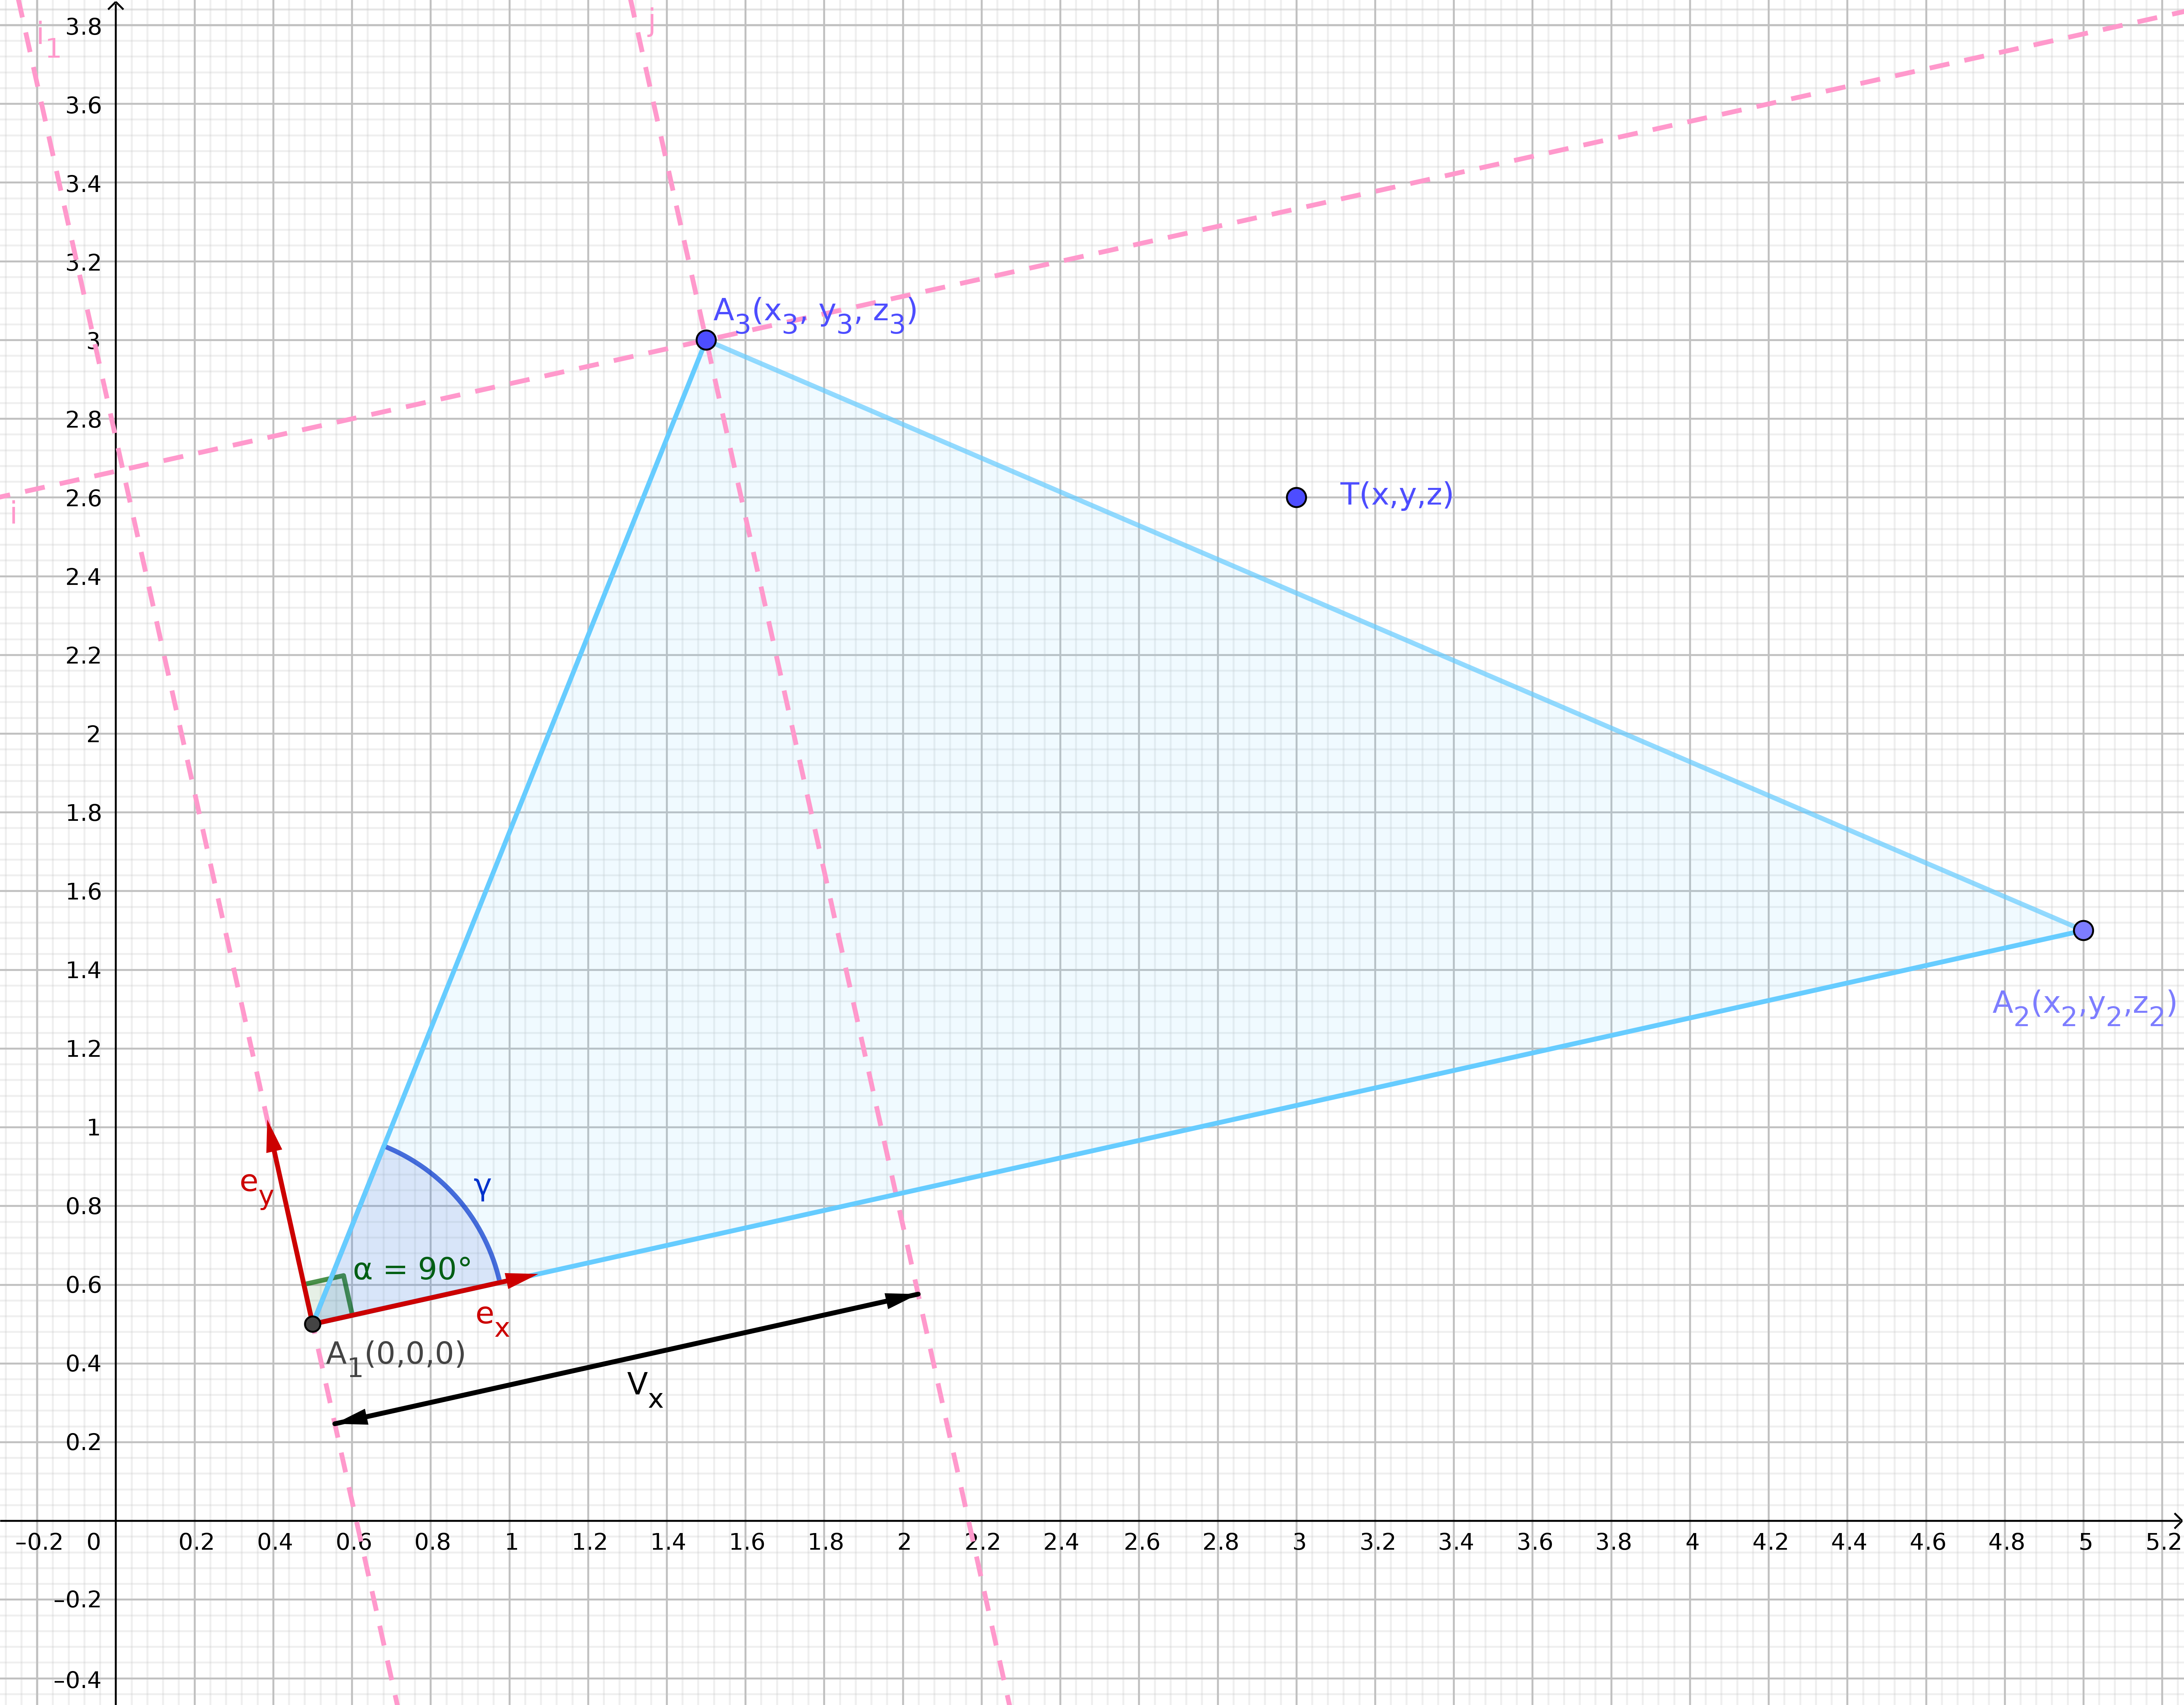
\includegraphics[width=0.8\textwidth]{multilateration.png}
                \caption{Multilateration in Euclidean space}
                \label{fig:multilateration}
            \end{figure}
    \end{columns}
    \begin{equation}
        \begin{split}
            &B_0(0,0,0) \\
            &B_1(U, 0, 0) = B_1(\Vert A_2 - A_1 \Vert, 0, 0) \\
            &B_2(V_x, V_y, 0) = B_2(\boldsymbol{e_x} \cdot (A_3 - A_1), \boldsymbol{e_y} \cdot (A_3 - A_1), 0) 
        \end{split}
        \label{eqn:multilateration_to_simplified_problem}
    \end{equation}
\end{frame}

\section{Ranging system architecture}

\section{Bluetooth mesh}

\section{Hardware}

\section{Software}

\section{System evaluation}

\section{Conclusion}

\end{document}